\documentclass[a4paper,10pt,twocolumn,english]{article}

% ============================================================================
% Packages
% ============================================================================

\usepackage{babel}
\usepackage[utf8]{inputenc}
\usepackage[T1]{fontenc}
\usepackage{lmodern}
\usepackage{amsmath,amssymb,amsthm,mathtools}
\usepackage{graphicx}
\usepackage{booktabs}
\usepackage{array}
\usepackage{longtable}
\usepackage{listings}
\usepackage{xcolor}
\usepackage{hyperref}
\usepackage{url}
\usepackage{enumitem}
\usepackage{microtype}
\usepackage{cleveref}
\usepackage[font=small,labelfont=bf]{caption}
\usepackage{tikz}

% Reduce space between section number and title, prevent hyphenation in headings
\makeatletter
\renewcommand{\@seccntformat}[1]{\csname the#1\endcsname\hspace{0.5em}}
\renewcommand{\section}{\@startsection{section}{1}{\z@}%
  {-3.5ex \@plus -1ex \@minus -.2ex}%
  {2.3ex}%
  {\raggedright\normalfont\large\bfseries}}
\renewcommand{\subsection}{\@startsection{subsection}{2}{\z@}%
  {-3.25ex \@plus -1ex \@minus -.2ex}%
  {1.5ex}%
  {\raggedright\normalfont\normalsize\bfseries}}
\renewcommand{\subsubsection}{\@startsection{subsubsection}{3}{\z@}%
  {-3.25ex \@plus -1ex \@minus -.2ex}%
  {1.5ex}%
  {\raggedright\normalfont\small\bfseries}}
\makeatother
\usetikzlibrary{positioning,calc,arrows.meta}

% TikZ figure styles
\tikzset{
  figfont/.style={font=\scriptsize\sffamily},
  figbox/.style={draw, rounded corners=2pt, align=center, inner sep=4pt},
  figboxgray/.style={figbox, fill=gray!10},
  figsubbox/.style={figbox, fill=white},
  figsubboxgray/.style={figbox, fill=gray!5},
  figarrow/.style={-{Stealth[length=2mm]}, thick},
  figarrowstrong/.style={figarrow, line width=0.6pt},
}

% ============================================================================
% Typography improvements
% ============================================================================

\raggedbottom                           % Consistent local spacing
\widowpenalty=10000                     % Prevent widows (single lines at top)
\clubpenalty=10000                      % Prevent orphans (single lines at bottom)
\displaywidowpenalty=10000              % Prevent widows after display math
\predisplaypenalty=50                   % Discourage break before display math
\postdisplaypenalty=50                  % Discourage break after display math
\setlength{\emergencystretch}{2em}      % Reduce overfull lines in narrow columns
\setlength{\columnsep}{16pt}            % Slightly wider gutter for two-column reading
\setlength{\parskip}{0pt plus 1pt}      % Flexible paragraph spacing
\setlength{\floatsep}{10pt plus 2pt minus 2pt}
\setlength{\textfloatsep}{12pt plus 2pt minus 2pt}
\setlength{\intextsep}{10pt plus 2pt minus 2pt}
\setlength{\tabcolsep}{4pt}
\renewcommand{\arraystretch}{1.08}
\renewcommand{\topfraction}{0.85}       % Allow more floats at top
\renewcommand{\bottomfraction}{0.85}    % Allow more floats at bottom
\renewcommand{\textfraction}{0.10}      % Require less text on float pages
\renewcommand{\floatpagefraction}{0.7}  % Fuller float pages
\setcounter{topnumber}{2}
\setcounter{bottomnumber}{1}
\setcounter{totalnumber}{3}
\setlist[itemize]{leftmargin=*, itemsep=2pt, topsep=3pt}
\setlist[enumerate]{leftmargin=*, itemsep=2pt, topsep=3pt}
\setlist[description]{leftmargin=0pt, labelindent=0pt, itemsep=2pt, topsep=3pt}

% ============================================================================
% Theorem environments
% ============================================================================

\theoremstyle{definition}
\newtheorem{definition}{Definition}[section]

\theoremstyle{plain}
\newtheorem{theorem}[definition]{Theorem}
\newtheorem{lemma}[definition]{Lemma}
\newtheorem{proposition}[definition]{Proposition}
\newtheorem{corollary}[definition]{Corollary}

\theoremstyle{definition}
\newtheorem{example}[definition]{Example}
\newtheorem{assumption}{Assumption Block}

\theoremstyle{remark}
\newtheorem{remark}[definition]{Remark}

% ============================================================================
% Custom commands
% ============================================================================

\newcolumntype{L}[1]{>{\raggedright\arraybackslash}p{#1}}

\newcommand{\Coherent}{\ensuremath{\mathsf{Coherent}}}
\newcommand{\EdgeCoherent}{\ensuremath{\mathsf{EdgeCoherent}}}
\newcommand{\ActiveEdge}{\ensuremath{\mathsf{ActiveEdge}}}
\newcommand{\Consume}{\ensuremath{\mathsf{Consume}}}
\newcommand{\GEnv}{\ensuremath{\mathsf{GEnv}}}
\newcommand{\DEnv}{\ensuremath{\mathsf{DEnv}}}
\newcommand{\Hbyz}{\ensuremath{H_{\mathrm{byz}}}}
\newcommand{\Obssafe}{\ensuremath{\mathsf{Obs}_{\mathrm{safe}}^{\mathrm{byz}}}}
\newcommand{\Eqsafe}{\ensuremath{\mathsf{Eq}_{\mathrm{safe}}^{\mathrm{byz}}}}
\newcommand{\Ebyz}{\ensuremath{\mathcal{E}_{\mathrm{byz}}}}
\newcommand{\ByzSafe}{\ensuremath{\mathsf{ByzSafe}}}
\newcommand{\ByzChar}{\ensuremath{\mathsf{ByzChar}}}
\newcommand{\wf}{\ensuremath{\mathsf{wf}}}
\newcommand{\consumeOne}{\ensuremath{\mathsf{consumeOne}}}
\newcommand{\RecvCompatible}{\ensuremath{\mathsf{RecvCompatible}}}
\newcommand{\EdgeShares}{\ensuremath{\mathsf{EdgeShares}}}
\newcommand{\ByzIfaceWF}{\ensuremath{\mathsf{ByzIfaceWF}}}

\newenvironment{citelist}{%
  \begin{list}{}{%
    \setlength{\leftmargin}{1.25em}%
    \setlength{\itemindent}{-1.25em}%
    \setlength{\itemsep}{2pt}%
    \setlength{\parsep}{0pt}%
    \setlength{\topsep}{3pt}}%
}{\end{list}}

\lstset{
  basicstyle=\ttfamily\footnotesize,
  keywordstyle=\color{blue},
  commentstyle=\color{gray},
  stringstyle=\color{red},
  breaklines=true,
  frame=single,
  columns=fullflexible,
  aboveskip=5pt,
  belowskip=5pt,
  xleftmargin=0pt,
  literate={->}{$\to$\ }2 {forall}{$\forall$}1 {:=}{$\coloneqq$}2
}

% ============================================================================
% Document
% ============================================================================

\title{Coherence for Asynchronous Buffered MPST:\\A Mechanized Metatheory}
\author{S. H. Berman}
\date{\empty}

\begin{document}
\maketitle

\begin{abstract}
Classical MPST uses coherence and projectability on global types to justify local safety. We define
an operational coherence invariant, $\Coherent(G,D)$, over projected local environments and buffered
traces, and show that this invariant is sufficient for preservation in asynchronous semantics. The
operational coherence invariant yields a reusable three-way edge split that avoids per-step global
re-derivation in our mechanized development. Lean~4 mechanization confirms the results under
parameterized delivery semantics.
\end{abstract}

% ============================================================================
\section{Introduction}
\label{sec:introduction}
% ============================================================================

\subsection{Background}

Multiparty session types guarantee that distributed protocols execute without communication errors.
The central technical challenge is preservation: showing that each protocol step maintains
well-typedness. Binary session types use duality for two-party compatibility. MPST generalizes this
with established global coherence and projectability conditions.

To address preservation, the MPST field has developed projection techniques that take a global
choreography to local session types. A global type specifies the full protocol. Projection then
extracts the local view for each participant. Safety means that local executions remain consistent
with their projected types.

Classical MPST coherence and projectability conditions are formulated at the global-type level (Honda,
Yoshida, and Carbone, 2008; Honda, Yoshida, and Carbone, 2016; Castagna et al., 2012), with later work
refining projection criteria (Majumdar et al., 2021).

In 2008, Honda et al.\ introduced asynchronous buffered MPST. Their preservation proof was organized
around global typing and projection consistency after transitions. Many later presentations keep this
global-first organization (Honda, Vasconcelos, and Kubo, 1998; Scalas and Yoshida, 2019), while
mechanized developments continue to refine proof organization and robustness (Tirore, Bengtson, and
Carbone, 2025).

Prior MPST literature formulates coherence at the global-type level through projectability and
well-formedness conditions. This paper refines coherence at the operational level by using
$\Coherent(G,D)$ over local environments and buffered traces. Our operational formulation makes
preservation local and compositional and removes the long-standing per-step global re-derivation
bottleneck. We confirm this result via Lean 4 mechanization.

\subsection{Insight}

Projection defines a quotient: it erases global structure while preserving safety-relevant information.
So the question becomes: what is the exact invariant that survives this erasure? We isolate an
operational form of coherence, $\Coherent(G,D)$, as the invariant required by our preservation proofs.
Binary session types use duality for two-party compatibility. This formulation instantiates n-ary
compatibility as receiver-buffer alignment at each active edge (Carbone et al., 2015).

Because $\Coherent(G,D)$ captures exactly what projection preserves for this proof architecture, it is
neither too strong nor too weak. This exactness enables compositionality. Local proofs on individual
edges combine to yield global preservation. No global re-derivation is required.

\subsection{Technical Approach}

Preservation reduces to a three-way case split over edges. For each edge, exactly one case applies:
directly updated, adjacent, or disjoint. Each case admits a focused local proof. After which, proofs
compose directly.

The local-to-global shape follows standard invariant methods from program logics (Reynolds, 2002;
O'Hearn, 2007), while aligning with the process-calculus decomposition tradition (Plotkin, 1981;
Milner, 1999).

\subsection{Scope and Claims}

This paper has two central claims. The first is Coherence preservation through a three-way split, which
applies uniformly across all transitions. The second is session evolution under subtype replacement via
\texttt{Consume\_mono}.

This is the first publication in a three-part series on asynchronous buffered semantics with
\texttt{DeliveryModel} parameterization. This paper defines the invariant kernel. The second paper
develops quantitative bounds and decision procedures on that kernel. The third paper proves
reconfiguration commutation and envelope exactness. Figure~1 shows the proof architecture.

Our contributions are as follows:
\begin{enumerate}
  \item A mechanized local preservation architecture using operational coherence over active edges and a reusable three-way edge split.
  \item A message-alignment proof kernel through \texttt{Consume} and the lemmas \texttt{Consume\_append} and \texttt{Consume\_cons}.
  \item A session-evolution theorem under asynchronous subtype replacement via \texttt{Consume\_mono}.
  \item A delivery-parametric mechanization profile with a typed effect bridge to the VM layer.
\end{enumerate}

\begin{figure}[tbp]
\centering
\resizebox{\columnwidth}{!}{%
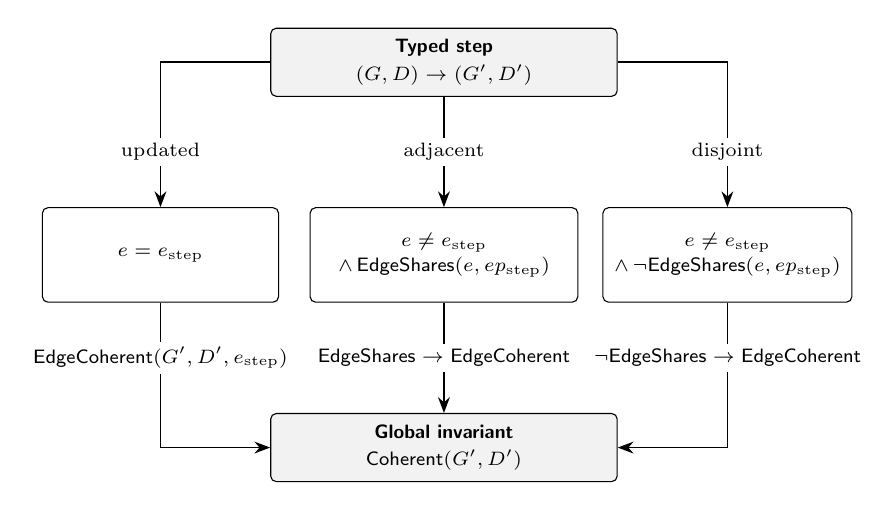
\begin{tikzpicture}[figfont]
  % Typed step at top
  \node[figboxgray, minimum width=44mm] (step)
    {\textbf{Typed step}\\[2pt] $(G,D)\to(G',D')$};

  % Three-way split: predicate boxes only (case names on arrows)
  \node[figsubbox, below=14mm of step, xshift=-36mm, minimum width=30mm, minimum height=12mm] (updated)
    {$e=e_{\mathrm{step}}$};
  \node[figsubbox, below=14mm of step, minimum width=34mm, minimum height=12mm] (shared)
    {$e\neq e_{\mathrm{step}}$\\[1pt] $\land\,\EdgeShares(e,ep_{\mathrm{step}})$};
  \node[figsubbox, below=14mm of step, xshift=36mm, minimum width=30mm, minimum height=12mm] (unrel)
    {$e\neq e_{\mathrm{step}}$\\[1pt] $\land\,\neg\EdgeShares(e,ep_{\mathrm{step}})$};

  \node[figboxgray, below=14mm of shared, minimum width=44mm] (global)
    {\textbf{Global invariant}\\[2pt] $\Coherent(G',D')$};

  % Labeled arrows from step to each case
  \draw[figarrowstrong] (step) -- (shared);
  \draw[figarrowstrong] (step.west) -- (updated.north |- step.west) -- (updated.north);
  \draw[figarrowstrong] (step.east) -- (unrel.north |- step.east) -- (unrel.north);
  % Arrow labels centered on vertical segments, same height
  % White fill creates clean break in arrow where text appears
  \coordinate (label-y-top) at ($(step.south)!0.5!(shared.north)$);
  \node[font=\scriptsize, fill=white, inner sep=2pt] at (updated |- label-y-top) {updated};
  \node[font=\scriptsize, fill=white, inner sep=2pt] at (shared |- label-y-top) {adjacent};
  \node[font=\scriptsize, fill=white, inner sep=2pt] at (unrel |- label-y-top) {disjoint};

  % Labeled arrows from cases to global invariant
  \draw[figarrowstrong] (updated.south) |- (global.west);
  \draw[figarrowstrong] (shared.south) -- (global.north);
  \draw[figarrowstrong] (unrel.south) |- (global.east);
  % Arrow labels centered on vertical segments, same height
  % White fill creates clean break in arrow where text appears
  \coordinate (label-y-bot) at ($(shared.south)!0.5!(global.north)$);
  \node[font=\scriptsize, fill=white, inner sep=2pt] at (updated |- label-y-bot) {$\EdgeCoherent(G',D',e_{\mathrm{step}})$};
  \node[font=\scriptsize, fill=white, inner sep=2pt] at (shared |- label-y-bot) {$\EdgeShares \to \EdgeCoherent$};
  \node[font=\scriptsize, fill=white, inner sep=2pt] at (unrel |- label-y-bot) {$\neg\EdgeShares \to \EdgeCoherent$};
\end{tikzpicture}
}%
\caption{Local-to-global preservation architecture.}
\label{fig:p1-preservation-architecture}
\vspace{7pt}
\end{figure}

% ============================================================================
\section{Model and Semantics}
\label{sec:model}
% ============================================================================

Configurations are represented by endpoint and edge environments. \GEnv{} maps endpoints to local types. \DEnv{} maps directed edges to buffered type traces. \texttt{Buffers} maps directed edges to runtime payload queues.

Table~1 records the model assumptions used for exact statements in this paper.

\begin{table}[tbp]
\centering
\small
\begin{tabular}{@{}L{0.55\columnwidth}L{0.4\columnwidth}@{}}
\toprule
\textbf{Assumption} & \textbf{Status} \\
\midrule
asynchronous buffered semantics & required \\
active-edge quantification & required \\
fair scheduling profile & assumed where stated \\
\texttt{DeliveryModel} param. & required \\
crash-stop and Byzantine claims & interface claim only \\
\bottomrule
\end{tabular}
\caption{Model assumptions for exact statements}
\end{table}

\begin{assumption}[Core Model Premises]
Core claims in this paper assume asynchronous buffered semantics, active-edge quantification, and \texttt{DeliveryModel} parameterization. Fair scheduling assumptions apply where stated.
\end{assumption}

\begin{definition}[Active Edge]
$\ActiveEdge(G, e)$ holds when both endpoints of edge $e$ are present in $G$.
\end{definition}

\begin{definition}[Edge Coherence]
$\EdgeCoherent(G, D, e)$ holds when the receiver side can consume the buffered trace on edge $e$ under the local type in $G$.
\end{definition}

\begin{definition}[Coherence]
$\Coherent(G, D)$ holds when every active edge is edge coherent.
\end{definition}

\begin{definition}[Consume]
$\Consume$ is the recursive alignment function that interprets buffered traces against receiver expectations.
\end{definition}

\begin{definition}[Byzantine Interface Well-Formedness]
$\ByzIfaceWF(G, D)$ is the interface predicate used for Byzantine-facing statements in this paper, and is mechanized as a definitional alias of $\Coherent(G, D)$.
\end{definition}

Delivery behavior is parameterized by \texttt{DeliveryModel}. This gives one theorem shape across FIFO, causal, and lossy instances.
\begin{figure}[tbp]
\centering
\footnotesize
\[
\begin{aligned}[t]
\Coherent(G,D)\ :=\ \forall e,\ \ActiveEdge(G,e)
\\
\to\ \EdgeCoherent(G,D,e).
\end{aligned}
\]
\vspace{-6pt}
\caption{Active-edge quantification boundary: only edges with present endpoints contribute coherence obligations.}
\label{fig:p1-active-edge-boundary}
\end{figure}
Edges incident to absent endpoints are excluded by $\ActiveEdge$.

Table~2 fixes notation used in this paper.

\begin{table}[tbp]
\centering
\small
\begin{tabular}{@{}L{0.4\columnwidth}L{0.55\columnwidth}@{}}
\toprule
\textbf{Symbol} & \textbf{Meaning} \\
\midrule
$\Hbyz$ & Byzantine characterization bundle \\
$\Obssafe$ & Byzantine safety-visible observation \\
$\Eqsafe$ & Byzantine safety-visible equality \\
$\Ebyz$ & Byzantine determinism-envelope \\
\Coherent & global active-edge compatibility \\
\EdgeCoherent & edge-local compatibility check \\
\Consume & trace-to-type alignment function \\
\ActiveEdge & endpoint-presence guard \\
\bottomrule
\end{tabular}
\caption{Notation}
\end{table}

\subsection{Why Coherence}

The term follows the linear-logic compatibility tradition from coherence-space semantics and session typing foundations, including Girard (1987), Caires and Pfenning (2010), and Wadler (2012). Usage in this paper is operational rather than denotational.

This operational usage is aligned with, but distinct from, classical MPST global coherence and projectability (Honda, Yoshida, and Carbone, 2008; Honda, Yoshida, and Carbone, 2016; Castagna et al., 2012) and logical n-ary coherence accounts (Carbone et al., 2015; Carbone et al., 2016; Carbone et al., 2017).

Operationally, our edge-local notion also sits in the lineage connecting session typing, subtyping, and communicating-automata views (Gay and Hole, 2005; Deni\'{e}lou and Yoshida, 2012; Brand and Zafiropulo, 1983).

The key structural correspondence is compatibility. A coherence-space token corresponds to an edge-local communication view, and a clique corresponds to a globally coherent configuration over active edges.

\begin{table}[tbp]
\centering
\small
\begin{tabular}{@{}L{0.38\columnwidth}L{0.57\columnwidth}@{}}
\toprule
\textbf{Coherence-space} & \textbf{MPST operational} \\
\midrule
token & directed edge with buffered trace \\
coherence relation & \texttt{EdgeCoherent} \\
clique & \texttt{Coherent} configuration \\
linear-map preservation & step preservation theorem \\
\bottomrule
\end{tabular}
\caption{Coherence-space correspondence}
\end{table}

% ============================================================================
\section{Worked Example}
\label{sec:example}
% ============================================================================

We use one running example throughout the paper.

\begin{example}[Single-Pool Capacity Session]
Roles are \texttt{C} (client), \texttt{P} (pool), and \texttt{M} (monitor), with global interaction:

\noindent\begin{minipage}{\columnwidth}
\begin{lstlisting}
C -> P : Request(n)
P -> C : Grant(k)
C -> M : Report(k)
M -> P : Confirm
P -> C : Token(t)
\end{lstlisting}
\end{minipage}

Fix local continuations:

\noindent\begin{minipage}{\columnwidth}
\begin{lstlisting}
L_C := recv P Grant(k);
       send M Report(k);
       recv P Token(t); end
L_P := recv M Confirm;
       send C Token(t); end
L_M := recv C Report(k);
       send P Confirm; end
\end{lstlisting}
\end{minipage}

and in-flight configuration $(G_0,D_0)$:

\noindent\begin{minipage}{\columnwidth}
\begin{lstlisting}
G_0(C) = L_C
G_0(P) = L_P
G_0(M) = L_M
D_0(P,C) = [Grant(k)]
D_0(e)   = []    for e != (P,C)
\end{lstlisting}
\end{minipage}

Assume typing judgment $\Gamma \vdash (G_0,D_0)\ \wf$.
\end{example}

The active-edge obligation is:
\[
\forall e,\ \ActiveEdge(G_0,e)\to \EdgeCoherent(G_0,D_0,e).
\]

The example is used via the following derived rule instances.

{\footnotesize
\[
\dfrac{
  \Gamma \vdash (G_0,D_0)\ \wf \quad D_0(P,C){=}[\mathrm{Grant}]
}{
  (G_0,D_0){\to}(G_1,D_1) \land \EdgeCoherent(G_1,D_1,e)
}
\]

\[
\dfrac{
  \Gamma \vdash (G_1,D_1)\ \wf \quad \mathsf{Consume\_append}
}{
  (G_1,D_1){\to}(G_2,D_2) \land \EdgeCoherent(G_2,D_2,e)
}
\]

\[
\dfrac{
  \Coherent(G_0,D_0) \quad \RecvCompatible(G_0,G'_0)
}{
  \Coherent(G'_0,D_0)
}
\]
}

For the step edge $u=(C,M)$, the case split used later is: updated ($e=u$), shared-endpoint ($e\neq u \land \EdgeShares(e,C\ \text{or}\ M)$), and unrelated ($e\neq u$ and no shared endpoint).

% ============================================================================
\section{Coherence Preservation Architecture}
\label{sec:preservation}
% ============================================================================

\begin{theorem}[Coherence Preservation]
\label{thm:coherence-preservation}
For all environments $G,D,G',D'$, if $(G,D) \to (G',D')$ is a well-typed step in the send and recv and select and branch fragment, then
\[
\Coherent(G,D) \implies \Coherent(G',D').
\]
This claim is exact for one-step preservation in the stated core rule fragment.
\end{theorem}

\begin{proof}[Proof sketch]
The argument is a reusable case-analysis pipeline over edges.

\begin{enumerate}
  \item Fix a typed one-step transition and an arbitrary edge $e$ that is active after the step.
  \item Apply \texttt{edge\_case\_split} to partition $e$ into:
  \begin{itemize}
    \item updated edge ($e = e_{\mathrm{step}}$),
    \item shared-endpoint edge ($e \neq e_{\mathrm{step}} \land \EdgeShares(e, ep_{\mathrm{step}})$),
    \item unrelated edge ($e \neq e_{\mathrm{step}} \land \neg \EdgeShares(e, ep_{\mathrm{step}})$).
  \end{itemize}
  \item Updated-edge case: send/recv/select/branch obligations are discharged by rule-local preservation lemmas; message-to-type alignment is reduced to \texttt{Consume\_append} (enqueue-facing) or \texttt{Consume\_cons} (dequeue-facing).
  \item Shared-endpoint case: use store/buffer irrelevance lemmas to show unaffected projections are preserved; transport pre-state $\EdgeCoherent$ to post-state $\EdgeCoherent$.
  \item Unrelated-edge case: apply frame-style transport (no touched endpoint, no touched buffer segment); conclude edge-local coherence is unchanged.
  \item Reassemble all cases to obtain $\Coherent(G',D')$.
\end{enumerate}

The same skeleton is used uniformly across send/recv/select/branch, which is the main proof-reuse gain in this paper.
\end{proof}

The split operator is implemented by \texttt{edge\_case\_split}. Rule-level preservation lemmas are grouped by send, recv, select, and branch cases. Table~4 gives the primary module map, and \cref{app:chains} records theorem-to-lemma chains with exact Lean anchors.

The architecture is quotient-first. The concrete step relation induces dynamics on equivalence classes once coherence-preserving symmetries are quotiented out.

The quotienting step should be read as symmetry reduction. Distinct interleavings that are equivalent under the symmetry relation are identified as one observable class. Formally, the induced square is:
\[
q(\mathsf{step}(C))\ =\ \mathsf{step}_{/ \sim}(q(C)).
\]

The square states the commuting condition used across these three papers. This paper establishes the preservation side needed to make the quotient dynamics well-defined.

\begin{figure}[tbp]
\centering
\scriptsize
\[
\begin{array}{c}
\text{checked edge }e\\[2pt]
\Downarrow\\[2pt]
\begin{array}{l}
\text{(updated)}\quad e=u\\
\text{(shared)}\quad e\neq u\land \EdgeShares(e,\mathit{ep})\\
\text{(unrelated)}\quad e\neq u\land \neg \EdgeShares(e,\mathit{ep})
\end{array}
\end{array}
\]
\vspace{-6pt}
\caption{Case partition used by \texttt{edge\_case\_split}: updated, shared-endpoint, and unrelated edges.}
\label{fig:p1-case-partition}
\end{figure}
The three branches are discharged by updated-edge preservation, shared-endpoint transport, and unrelated-edge frame transport, respectively.

% ============================================================================
\section{Message-Type Alignment via Consume}
\label{sec:consume}
% ============================================================================

$\Consume$ is the proof kernel for message-type alignment. It removes most rule-specific structural complexity from preservation proofs.

\begin{lemma}[Consume\_append]
Consumption over concatenated traces factors through sequential consumption.
\end{lemma}

\begin{lemma}[Consume\_cons]
Head consumption reduces to one-step alignment plus recursive continuation alignment.
\end{lemma}

\begin{proof}[Proof sketch]
The library is centered on $\consumeOne$ and structural recursion on trace shape.

\begin{enumerate}
  \item \texttt{Consume\_append}: induction on trace prefix $ts$; base case $ts = []$ is immediate by simplification ($L' = L_r$); step case peels one $\consumeOne$ transition and applies induction hypothesis to the residual local type.
  \item \texttt{Consume\_cons}: unfold one $\Consume$ step on head $T$; case split on $\consumeOne(\mathit{from}, T, L_r)$; resulting equation is definitional in both branches.
  \item Preservation integration: send/select proofs use \texttt{Consume\_append} to justify extending buffered traces; recv/branch proofs use \texttt{Consume\_cons} to justify consuming the head message and continuing.
\end{enumerate}

This isolates alignment complexity into two reusable lemmas rather than duplicating ad-hoc trace reasoning in each operational rule.
\end{proof}

For the worked example, \texttt{Consume\_cons} discharges the \texttt{Grant} receive step at \texttt{C} by reducing the obligation to continuation coherence after one aligned message.

% ============================================================================
\section{Session Evolution via Subtyping}
\label{sec:evolution}
% ============================================================================

Session evolution replaces one endpoint local type with a compatible refinement and asks whether coherence is preserved.

This replacement argument follows a standard commutation intuition from trace-equivalence and commuting-conversion lines. The standard point is that local reorderings or local refinements should preserve observable behavior when compatibility conditions hold. What is new here is an operational criterion for asynchronous subtype replacement that is stated directly through \texttt{Consume\_mono} and discharged with edge-local coherence obligations.

\begin{assumption}[Replacement Compatibility]
The subtype-evolution theorem assumes endpoint replacement at $ep$ satisfies typing-domain preservation, receive-side monotonicity side conditions, and environment consistency for unaffected endpoints.
\end{assumption}

\begin{theorem}[Session Evolution via \texttt{Consume\_mono}]
\label{thm:session-evolution}
For all endpoints $ep$ and environments $G,D,G_{\mathrm{rep}}$, if Assumption Block~1 holds for replacement at $ep$, then
\[
\Coherent(G,D) \implies \Coherent(G_{\mathrm{rep}},D).
\]
This claim is exact for type replacement steps covered by Assumption Block~1.
\end{theorem}

\begin{proof}[Proof sketch]
The replacement theorem is proved by a monotonicity-to-global-lift chain.

\begin{enumerate}
  \item Local monotonicity: establish receive-compatibility ($\RecvCompatible$) between old and replacement local types; apply \texttt{Consume\_mono} to show every successful old consumption remains successful after replacement.
  \item Edge lift: use \texttt{EdgeCoherent\_type\_replacement} on edges targeting the replaced endpoint; for non-target edges, transport coherence by environment agreement.
  \item Global lift: combine edge cases to derive \texttt{Coherent\_type\_replacement}.
  \item Progress compatibility: use liveness-side lemmas (\texttt{progress\_conditions\_type\_replacement}) to preserve operational side conditions.
\end{enumerate}

Hence compatible subtype replacement preserves Coherence without re-running global derivations.
\end{proof}

Core lemmas are in the subtype-replacement core and liveness layers.
\begin{figure}[tbp]
\centering
\footnotesize
\[
\begin{aligned}[t]
\Coherent(G,D)\ \land\ \mathsf{Compat}_{ep}(G,G_{\mathrm{rep}})
\\
\Longrightarrow\ \Coherent(G_{\mathrm{rep}},D)
\end{aligned}
\]
\[
\texttt{Consume\_mono}\ \Longrightarrow\ \text{edge lift}\ \Longrightarrow\ \text{global lift}
\]
\vspace{-8pt}
\caption{Subtype-replacement commutation principle and proof-lift chain.}
\label{fig:p1-replacement-commutation}
\end{figure}
with compatibility discharged by \texttt{Consume\_mono} and replacement side conditions.

% ============================================================================
\section{Mechanization Summary}
\label{sec:mechanization}
% ============================================================================

Table~4 maps each core claim to concrete modules and representative theorem anchors.

\begin{table}[tbp]
\centering
\footnotesize
\begin{tabular}{@{}L{0.27\columnwidth}L{0.36\columnwidth}L{0.27\columnwidth}@{}}
\toprule
\textbf{Claim} & \textbf{Modules} & \textbf{Anchors} \\
\midrule
Definitions & Consume.lean, EdgeCoherence\-Core.lean & Consume, Edge\-Coherent \\
Consume kernel & Consume.lean & Consume\_append \\
Three-way split & Unified.lean & edge\_case\_split \\
Preservation & Preservation*.lean & Coherent\_*\_preserved \\
Delivery variants & DeliveryModel.lean & *Delivery\_laws \\
Subtype repl. & SubtypeReplacement*.lean & Consume\_mono \\
\bottomrule
\end{tabular}
\caption{Claim to artifact mapping}
\end{table}

% ============================================================================
\section{Effect-Typed Bridge}
\label{sec:bridge}
% ============================================================================

\texttt{EffectSpec.handlerType} records typed effect obligations at the VM boundary. Runtime typing uses these obligations in the VM execution layer.

\begin{proposition}[Bridge Soundness]
For any selected handler $h$, if choreography obligations for $h$ are discharged and \texttt{EffectSpec.handlerType} holds for $h$, then VM-side typing obligations generated from $h$ are satisfied in the corresponding runtime instruction layer.
\end{proposition}

\begin{proof}[Proof sketch]
Let $h$ satisfy choreography-side obligations and \texttt{EffectSpec.handlerType}. Use the monitor contracts \texttt{monitor\_sound} and \texttt{unified\_monitor\_preserves} for the instruction sequence generated from $h$ to obtain preservation of VM typing obligations at runtime transitions for that handler fragment. Compose with the configuration-equivalence/effect-bisimulation bridge to transfer this local typing fact to the observational interface. Hence VM obligations generated from $h$ are satisfied.
\end{proof}

\begin{table}[tbp]
\centering
\small
\begin{tabular}{@{}L{0.45\columnwidth}L{0.5\columnwidth}@{}}
\toprule
\textbf{Bridge item} & \textbf{Role} \\
\midrule
choreography obligation & source protocol obligation \\
effect handler typing & typed executable obligation \\
VM runtime typing check & enforcement layer \\
\bottomrule
\end{tabular}
\caption{Bridge intent}
\end{table}

\begin{assumption}[Byzantine Interface Premises]
The interface statements in this section assume shared notation for $\Hbyz$, $\Obssafe$, $\Eqsafe$, and $\Ebyz$, plus theorem-pack capability naming consistency between abstract and runtime layers.
\end{assumption}

\begin{theorem}[Byzantine Interface Well-Formedness (BZ-1)]
Under Assumption Block~2, Byzantine safety-track statements in this paper are interpreted on configurations $(G,D)$ satisfying $\ByzIfaceWF(G,D)$ (definitional alias of $\Coherent(G,D)$). For any active edge, this interface yields the same sender-existence and $\Consume$ obligations as the Coherence layer.
\end{theorem}

\begin{corollary}[Dropped-Assumption Witness Interface (BZ-1.1)]
Let $\mathcal{A}$ be any assumption class named in $\Hbyz$. If a later construction provides a witness violating $\ByzSafe$ when $\mathcal{A}$ is dropped, then that witness can be expressed against the same active-edge Coherence interface used in this paper.
\end{corollary}

\begin{proposition}[Capability-Gated VM Interface (BZ-1.2)]
If a runtime profile includes Byzantine characterization and envelope-adherence capability evidence, then safety-visible runtime obligations are interpreted through $\Eqsafe$ modulo $\Ebyz$, and profile admission is blocked when required evidence is absent.
\end{proposition}

% ============================================================================
\section{Related Work}
\label{sec:related}
% ============================================================================

Binary duality and global re-derivation lines established important foundations for session safety (Honda, Yoshida, and Carbone, 2008; Honda, Yoshida, and Carbone, 2016). Classical global coherence and projectability accounts are developed and refined in global-type work (Castagna et al., 2012; Majumdar et al., 2021). Logical accounts frame coherence as n-ary duality or proof compatibility (Carbone et al., 2015; Carbone et al., 2016; Carbone et al., 2017), while data-dependent MPST extensions remain in the same global-projection discipline (Toninho et al., 2017).

We do not introduce coherence as a new MPST notion. Instead, we give a local operational reformulation of coherence that is tailored to mechanized asynchronous preservation.

Alternative local-first or rely/guarantee lines avoid standard global coherence checks and motivate contrast with global-first formulations (Scalas and Yoshida, 2018). Program-logical lines such as Actris operate at a different verification layer and target program proofs over protocol resources (Hinrichsen et al., 2020). Event-structure and partial-order lines provide alternate macro views of concurrency (Castellan et al., 2023).

Broader background includes process-calculus and communication-structure foundations (Hoare, 1985; Milner, 1999), programming-language typing baselines (Pierce, 2002), and model-checking perspectives on state-space reasoning (Baier and Katoen, 2008).

The main difference from prior work is a single local invariant kernel with a reusable proof split and a monotonic evolution theorem.

\begin{table}[tbp]
\centering
\small
\begin{tabular}{@{}L{0.47\columnwidth}L{0.48\columnwidth}@{}}
\toprule
\textbf{Prior limitation} & \textbf{Contribution} \\
\midrule
preservation tied to global re-derivation & reusable edge-local skeleton \\
weak theory/execution boundary & explicit effect-typed bridge \\
FIFO-centric semantics & one theorem under \texttt{DeliveryModel} \\
fragmented proof structure & split kernel + \texttt{Consume} lemmas \\
\bottomrule
\end{tabular}
\caption{Comparison with prior work}
\end{table}

% ============================================================================
\section{Limitations and Scope}
\label{sec:limitations}
% ============================================================================

This paper proves preservation-style safety only: active-edge coherence is preserved for the core asynchronous rule family, and coherence is stable under subtype replacement when replacement preserves typing domains, satisfies receive-side monotonicity, and keeps unaffected endpoints environment-consistent.

Quantitative, fault-characterization, and envelope-level claims are proved in later papers within this series.

% ============================================================================
\section{Conclusion}
\label{sec:conclusion}
% ============================================================================

Since Honda et al.\ (2008), many preservation accounts for asynchronous MPST have been organized around global re-derivation after each step. This paper gives a mechanized alternative.

The key insight is that projection from global to local types defines an erasure. The operational invariant $\Coherent(G,D)$ is exact for our preservation architecture. Because it is exact at the operational boundary, local proofs compose without global re-derivation.

The resulting kernel is small, compositional, and extensible. It supports subtype-driven session evolution through a single monotonicity lemma. The mechanization in Lean~4 confirms that the architecture scales.

% ============================================================================
\section*{Works Cited}
% ============================================================================

\begin{citelist}
\item Baier, C., and Katoen, J.-P. (2008). Principles of Model Checking. MIT Press.
\item Brand, D., and Zafiropulo, P. (1983). On Communicating Finite-State Machines. Journal of the ACM, 30(2), 323--342.
\item Caires, L., and Pfenning, F. (2010). Session Types as Intuitionistic Linear Propositions. CONCUR 2010.
\item Carbone, M., Lindley, S., Montesi, F., Sch\"urmann, C., and Wadler, P. (2016). Coherence Generalises Duality: A Logical Explanation of Multiparty Session Types. CONCUR 2016.
\item Carbone, M., Montesi, F., Sch\"urmann, C., and Yoshida, N. (2015). Multiparty Session Types as Coherence Proofs. CONCUR 2015.
\item Carbone, M., Montesi, F., Sch\"urmann, C., and Yoshida, N. (2017). Multiparty Session Types as Coherence Proofs. Acta Informatica, 54(3), 243--269.
\item Castagna, G., Dezani-Ciancaglini, M., Gesbert, N., and Padovani, L. (2012). On Global Types and Multi-Party Sessions.
\item Castellan, S., et al. (2023). Event-structure and partial-order semantics for session-based concurrency. Journal of Logic and Algebraic Methods in Programming.
\item Cover, T. M., and Thomas, J. A. (2006). Elements of Information Theory (2nd ed.). Wiley.
\item Deni\'{e}lou, P.-M., and Yoshida, N. (2012). Multiparty Session Types Meet Communicating Automata. ESOP 2012.
\item Gay, S. J., and Hole, M. (2005). Subtyping for Session Types in the Pi Calculus. Acta Informatica, 42(2--3), 191--225.
\item Girard, J.-Y. (1987). Linear Logic. Theoretical Computer Science, 50(1), 1--101.
\item Hinrichsen, J., et al. (2020). Actris: Session-type based reasoning in separation logic. POPL 2020.
\item Hoare, C. A. R. (1985). Communicating Sequential Processes. Prentice Hall.
\item Honda, K. (1993). Types for Dyadic Interaction. CONCUR 1993.
\item Honda, K., Vasconcelos, V. T., and Kubo, M. (1998). Language Primitives and Type Discipline for Structured Communication-Based Programming. ESOP 1998.
\item Honda, K., Yoshida, N., and Carbone, M. (2008). Multiparty Asynchronous Session Types. POPL 2008.
\item Honda, K., Yoshida, N., and Carbone, M. (2016). Multiparty Asynchronous Session Types. Journal of the ACM, 63(1), Article 9.
\item Majumdar, R., Mukund, M., Stutz, F., and Zufferey, D. (2021). Generalising Projection in Asynchronous Multiparty Session Types. CONCUR 2021.
\item Milner, R. (1999). Communicating and Mobile Systems: The Pi-Calculus. Cambridge University Press.
\item Milner, R., Parrow, J., and Walker, D. (1992). A Calculus of Mobile Processes, I and II. Information and Computation, 100(1), 1--77.
\item O'Hearn, P. W. (2007). Resources, Concurrency, and Local Reasoning. Theoretical Computer Science, 375(1--3), 271--307.
\item Pierce, B. C. (2002). Types and Programming Languages. MIT Press.
\item Plotkin, G. D. (1981). A Structural Approach to Operational Semantics. DAIMI FN-19.
\item Reynolds, J. C. (2002). Separation Logic: A Logic for Shared Mutable Data Structures. LICS 2002.
\item Scalas, A., and Yoshida, N. (2018). Multiparty Session Types, Beyond Duality. Journal of Logical and Algebraic Methods in Programming, 97, 55--84.
\item Shannon, C. E. (1948). A Mathematical Theory of Communication. Bell System Technical Journal, 27(3), 379--423 and 27(4), 623--656.
\item Tirore, L., Bengtson, J., and Carbone, M. (2025). Mechanized MPST metatheory with subject-reduction robustness analysis. ECOOP 2025.
\item Toninho, B., and Yoshida, N. (2017). Certifying Data in Multiparty Session Types. Journal of Logical and Algebraic Methods in Programming, 90, 61--83.
\item Wadler, P. (2012). Propositions as Sessions. ICFP 2012.
\end{citelist}

% ============================================================================
\appendix
% ============================================================================

\section{Syntax and Judgments}
\label{app:syntax}

This appendix fixes the formal objects and judgment forms used in Sections~2--6.

\subsection{Roles, Endpoints, and Edges}

Let \texttt{Role} be the finite set of role names. An endpoint is a pair $(\mathit{sid},r)$ of session identifier and role. A directed edge is a triple $(\mathit{sid}, r_s, r_r)$ with sender role $r_s$ and receiver role $r_r$.

We write:
\begin{itemize}
  \item $\mathsf{src}(e)$ for the sender endpoint of edge $e$,
  \item $\mathsf{dst}(e)$ for the receiver endpoint of edge $e$,
  \item $\mathsf{role}(ep)$ for the role component of endpoint $ep$,
  \item $\EdgeShares(e, ep)$ when endpoint $ep$ is either $\mathsf{src}(e)$ or $\mathsf{dst}(e)$.
\end{itemize}

\subsection{Local Types and Environments}

Local types are generated by:

\noindent\begin{minipage}{\columnwidth}
\begin{lstlisting}
L ::= end
    | send r T L
    | recv r T L
    | select r {li : Li}i
    | branch r {li : Li}i
    | mu L
\end{lstlisting}
\end{minipage}

A typing environment $G$ maps endpoints to local types. A delayed-trace environment $D$ maps directed edges to buffered type traces.

\subsection{Active Edges and Coherence}

An edge is active exactly when both its endpoints are present in $G$:

\noindent\begin{minipage}{\columnwidth}
\begin{lstlisting}
ActiveEdge G e := (G (src e) != none) and (G (dst e) != none)
\end{lstlisting}
\end{minipage}

Edge coherence is a local receive-side compatibility judgment:

\noindent\begin{minipage}{\columnwidth}
\begin{lstlisting}
EdgeCoherent G D e :=
  exists Lr,
    G (dst e) = some Lr and
    Consume (role (src e)) Lr (D e) != none
\end{lstlisting}
\end{minipage}

Global coherence is active-edge quantification:

\noindent\begin{minipage}{\columnwidth}
\begin{lstlisting}
Coherent G D := forall e, ActiveEdge G e -> EdgeCoherent G D e
\end{lstlisting}
\end{minipage}

\section{Theorem-to-Lemma Chains and Lean Anchors}
\label{app:chains}

This appendix records compact proof skeletons for theorem-level claims and the exact Lean anchors used by each chain.

\subsection{Theorem 1: Coherence Preservation}

\textbf{Lemma chain.}
\begin{enumerate}
  \item Partition each checked edge by \texttt{edge\_case\_split}.
  \item Discharge updated-edge obligations by rule-local preservation lemmas.
  \item Discharge alignment obligations by \texttt{Consume\_append} and \texttt{Consume\_cons}.
  \item Reassemble to global active-edge quantification for \texttt{Coherent}.
\end{enumerate}

\textbf{Exact Lean anchors.}
\begin{itemize}
  \item \nolinkurl{lean/Protocol/Coherence/Unified.lean}: \texttt{edge\_case\_split}
  \item \nolinkurl{lean/Protocol/Coherence/Preservation.lean}: \texttt{Coherent\_send\_preserved}
  \item \nolinkurl{lean/Protocol/Coherence/PreservationRecv.lean}: \texttt{Coherent\_recv\_preserved}
  \item \nolinkurl{lean/Protocol/Coherence/SelectPreservation.lean}: \texttt{Coherent\_select\_preserved}, \texttt{Coherent\_branch\_preserved}
  \item \nolinkurl{lean/Protocol/Coherence/Consume.lean}: \texttt{Consume\_append}, \texttt{Consume\_cons}
\end{itemize}

\subsection{Theorem 2: Session Evolution via \texttt{Consume\_mono}}

\textbf{Lemma chain.}
\begin{enumerate}
  \item Establish receive-compatibility premise at the replacement endpoint.
  \item Lift consumption success along replacement by \texttt{Consume\_mono}.
  \item Lift edge-local replacement by \texttt{EdgeCoherent\_type\_replacement}.
  \item Lift globally by \texttt{Coherent\_type\_replacement}; preserve progress side conditions.
\end{enumerate}

\textbf{Exact Lean anchors.}
\begin{itemize}
  \item \nolinkurl{lean/Protocol/Coherence/SubtypeReplacementCore.lean}: \texttt{Consume\_mono}, \texttt{EdgeCoherent\_type\_replacement}, \texttt{Coherent\_type\_replacement}
  \item \nolinkurl{lean/Protocol/Coherence/SubtypeReplacementLiveness.lean}: \texttt{progress\_conditions\_type\_replacement}
\end{itemize}

\subsection{Proposition 1: Bridge Soundness}

\textbf{Lemma chain.}
\begin{enumerate}
  \item Use monitor contracts for handler-generated instructions.
  \item Lift effect-bisim facts to observational equivalence.
  \item Identify configuration-equivalence with the same silent effect-bisim class.
\end{enumerate}

\textbf{Exact Lean anchors.}
\begin{itemize}
  \item \nolinkurl{lean/Runtime/VM/Runtime/Monitor.lean}: \texttt{monitor\_sound}, \texttt{unified\_monitor\_preserves}
  \item \nolinkurl{lean/Runtime/Proofs/EffectBisim/Bridge.lean}: \texttt{effectBisim\_implies\_observationalEquivalence}
  \item \nolinkurl{lean/Runtime/Proofs/EffectBisim/ConfigEquivBridge.lean}: \texttt{configEquiv\_iff\_effectBisim\_silent}
\end{itemize}

\subsection{Theorem BZ-1: Byzantine Interface Well-Formedness}

\textbf{Lemma chain.}
\begin{enumerate}
  \item Expand \texttt{ByzIfaceWF} as definitional \texttt{Coherent}.
  \item On each active edge, extract sender witness and \texttt{Consume} success.
\end{enumerate}

\textbf{Exact Lean anchors.}
\begin{itemize}
  \item \nolinkurl{lean/Runtime/Proofs/Adapters/Distributed/EnvelopeTheorems.lean}: \texttt{ByzIfaceWF}, \texttt{byzIfaceWF\_iff\_coherent}, \texttt{bz1\_byzantineInterfaceWellFormedness}
\end{itemize}

\subsection{Proposition BZ-1.2: Capability-Gated VM Interface}

\textbf{Lemma chain.}
\begin{enumerate}
  \item Gate runtime operation by theorem-pack capability evidence.
  \item Extract Byzantine envelope adherence from witness evidence.
  \item Package cross-target conformance under the same envelope interface.
\end{enumerate}

\textbf{Exact Lean anchors.}
\begin{itemize}
  \item \nolinkurl{lean/Runtime/Proofs/TheoremPack/API.lean}: \texttt{canOperateUnderByzantineEnvelope}
  \item \nolinkurl{lean/Runtime/Proofs/Adapters/Distributed/EnvelopeTheorems.lean}: \texttt{vmByzantineEnvelopeAdherence\_of\_witness}, \texttt{byzantineCrossTargetConformance\_of\_witnesses}
\end{itemize}

\section{Delivery Parametricity and Runtime Bridge}
\label{app:delivery}

Preservation is parametric over \texttt{ConsumeM} laws. Required laws are: \texttt{nil}, \texttt{append}, \texttt{cons}, and renaming stability under endpoint-preserving renamings.

\section{Reproducibility}
\label{app:reproducibility}

Reproduction uses the repository-pinned Lean toolchain and manifest.

\begin{enumerate}
  \item Build paper modules via \texttt{lake build}.
  \item Run project checks \texttt{just escape} and \texttt{just verify-protocols}.
  \item Confirm theorem anchors resolve in the built environment.
\end{enumerate}

\section{Index of Main Results}
\label{app:index}

\begin{center}
\footnotesize
\begin{tabular}{@{}L{0.2\columnwidth}L{0.08\columnwidth}L{0.3\columnwidth}L{0.32\columnwidth}@{}}
\toprule
\textbf{Claim} & \textbf{Sec.} & \textbf{Assumption} & \textbf{Location} \\
\midrule
Theorem 1 & \S4 & Block 0 + core & Preservation*.lean \\
Theorem 2 & \S6 & Block 1 compat. & SubtypeRepl*.lean \\
Prop.\ 1 & \S8 & Block 0 + oblig. & runtime bridge \\
Thm.\ BZ-1 & \S8 & Block 2 iface & EnvelopeThms.lean \\
Cor.\ BZ-1.1 & \S8 & Block 2 + wit. & derived \\
Prop.\ BZ-1.2 & \S8 & Block 2 + gate & TheoremPack/*.lean \\
\bottomrule
\end{tabular}
\captionof{table}{Index of main results}
\end{center}

\end{document}
